\section{Постановка задачи}
Составьте алгоритм и напишите соответствующую ему программу, позволяющую
\begin{itemize}
    \item возводить целое число в квадрат;
    \item возводить натуральное число в натуральную степень;
    \item вычислять целую часть квадратного корня из натурального числа;
    \item вычислять целую часть кубического корня из натурального числа.
\end{itemize}


\clearpage
\section{Используемые инструменты}
Для решения вышеуказанной задачи были использованы следующие инструменты:
\begin{itemize}
    \item Основным ЯП был выбран Python версии 3.9.2;
    \item Для компиляции программы в бинарный файл .exe использован конвертер файлов Auto PY to EXE,
    который использует для своей работы PyInstaller.
\end{itemize}


\clearpage
\section{Общая структура библиотеки целых\\длинных чисел}
В библиотеке целых длинных содержится класс <<BigInt>>, внутри которого находятся следующие методы:
\begin{itemize}
    \item Выделение корня любой положительной целой степени из длинного целого числа.\\
    Программная реализация представляет подбор наиболее близкого числа, возведенного в данную из аргументов степень,
    при котором результат возведения в степень не будет превышать число, из которого выделяется корень.
    Выбор данного способа обусловлен простотой его реализации;
    \item Возведение в степень длинного целого числа.\\
    Программная реализация представляет бинарный алгоритм возведения числа в степень натурального числа.
    Первая реализация была сделана на основе рекурсивного умножения числа само на себя,
    но такой алгоритм оказался медленнее бинарного алгоритма возведения в степень.
\end{itemize}

Класс <<BigInt>> содержит в себе два основных поля:
\begin{enumerate}
    \item Поле хранения числа <<value>>.\\
    Представляет собой переменную типа строка, в котором содержится число экземпляра класса;
    \item Поле хранения знака числа <<is\_neg>>.\\
    Представляет собой переменную типа bool, в которой содержится информация о знаке числа.
    Значение True эквивалентно отрицательному числу, значение False - положительному;
\end{enumerate}

Создания экземпляра класса <<BigInt>> происходит следующие способами:
\begin{itemize}
    \item Создание экземпляра класса без передачи аргументов. Числовое значение такого экземпляра будет равно нулю.
    \begin{lstlisting}
a = BigInt()\end{lstlisting}
    \item Создание экземпляра класса с передачей в аргумент строки, которая может валидно быть приведена к типу целого числа.
    \begin{lstlisting}
a = BigInt('-1234567890')  # a = -1234567890
b = BigInt('1234567890')   # b = 1234567890
d = BigInt('0')            # d = 0\end{lstlisting}
    \item Создание экземпляра класса с передачей в аргумент целого числа.
    \begin{lstlisting}
a = BigInt(-1234567890)  # a = -1234567890
b = BigInt(1234567890)   # b = 1234567890
d = BigInt(0)            # d = 0\end{lstlisting}
    \item Создание экземпляра класса с передачей в аргумент экземпляра класса <<BigInt>>.
    \begin{lstlisting}
a = BigInt(-1234567890)  # a = -1234567890
b = BigInt(a)            # b = -1234567890\end{lstlisting}
\end{itemize}


\clearpage
\section{Примеры работы библиотеки}
В качестве примера работы будут использоваться прямые вызовы методов класса <<BigInt>>.

Пусть даны два целых длинных числа $a$ и $b$, сохраненных в экземпляр класса <<BigInt>>.
А так же, создадим экземпляр класса <<BigInt>> с нулевым значением.
    \begin{lstlisting}
a = BigInt('-1234567890987654321')
b = BigInt('9876543210123456789')
zero = BigInt()\end{lstlisting}

    \begin{itemize}
        \item Выполняем возведение в степень:
        \begin{lstlisting}
print(a.bipow(20))\end{lstlisting}
        Вывод:\\
        $67654945781131788253399139476950939867213847384221510782372183$
        $38736383554932818216005379411615896402318839463975841663187950$
        $47266740645217094738013218419327830527872057771151857381511749$
        $91352856101226216668855950857925749095871686783571452199421977$
        $46524667992025003348862025953101533163689052346013027443912327$
        $3028907724064631250587670777171351261244651206462401$
        \item Выполняем возведение в степень ноль:
        \begin{lstlisting}
print(b.bipow(0))\end{lstlisting}
        Вывод: $1$
        \item Выполняем извлечение корня:
        \begin{lstlisting}
print(b.birt(9))\end{lstlisting}
        Вывод: $128$
    \end{itemize}

\clearpage
\section{Вывод}
Мною был составлен алгоритм (в виде блок-схемы) и написана на языке Python программа, позволяющая:
\begin{itemize}
    \item возводить натуральное число в натуральную степень;
    \item вычислять целую часть $n$-го корня из натурального числа.
\end{itemize}

\clearpage
\section{Блок-схема методов библиотеки}
Ниже представлены блок-схемы методов в следующем порядке:
\begin{enumerate}
    \item Метод возведения натурального числа в натуральную степень с помощью бинарного алгоритма;
    \item Метод возведения натурального числа в натуральную степень с рекурсивного алгоритма (не используемый в программе);
    \item Метод вычисления целой части $n$-го корня из натурального числа.
\end{enumerate}
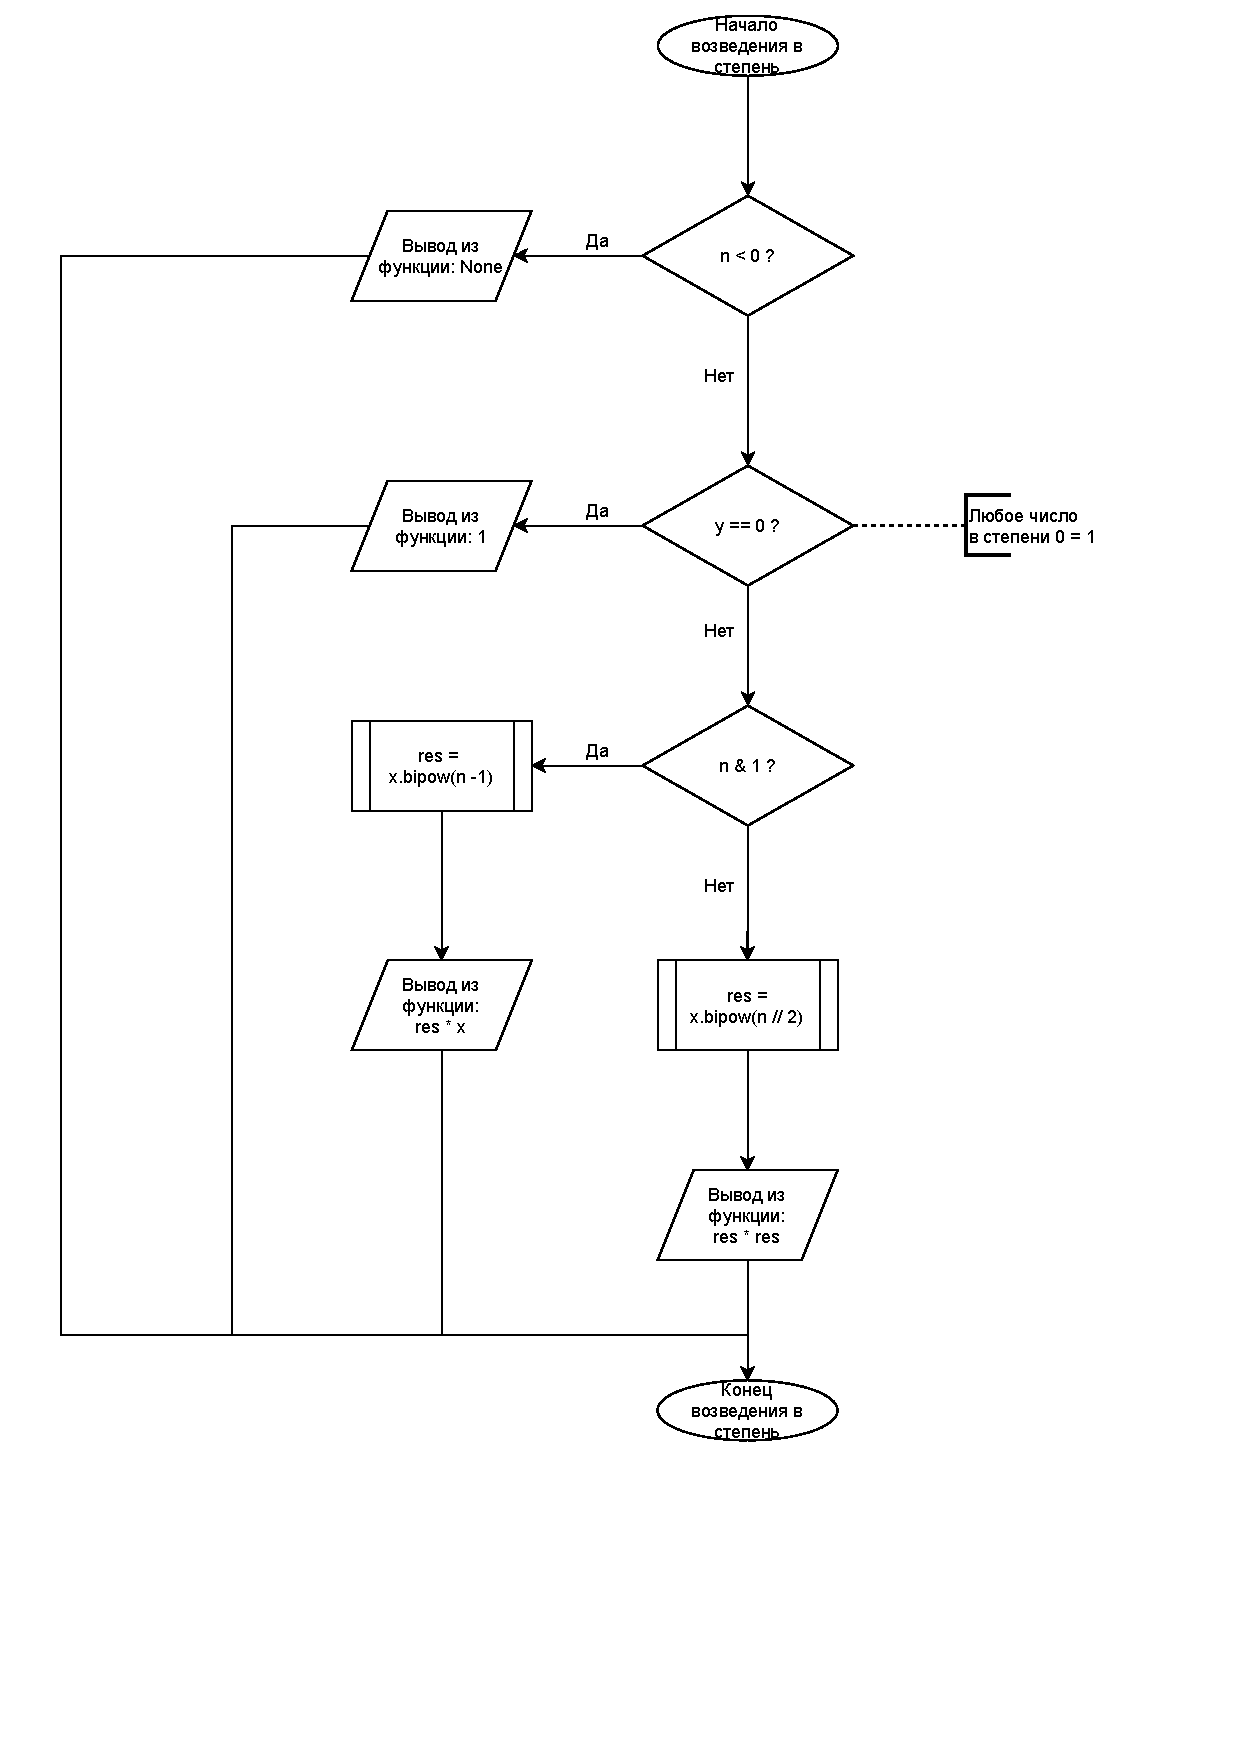
\includepdf[pages=-]{./Flowchart.pdf}
